\section{Boosting}

\begin{frame}{Boosting}
\begin{itemize}
    \item 思想:希望能有一种方法能够聚合多个弱学习器(每个弱学习器可以只比随机猜测表现好一点),使得整体学习器的性能更好。
    \item 一次性学习强学习器可能计算复杂度上承担不起,但每个弱学习器的计算复杂度较低,聚合多个弱学习器的计算复杂度可以接受。
\end{itemize}
\end{frame}

\begin{frame}{AdaBoost (a.k.a Adaptive Boosting)}
\begin{itemize}
    \item AdaBoost是最典型的boosting算法。
    \item AdaBoost 思想:在简单假设类上构建线性预测期作为更强大的假设类。
\end{itemize}
算法:
\begin{center}
    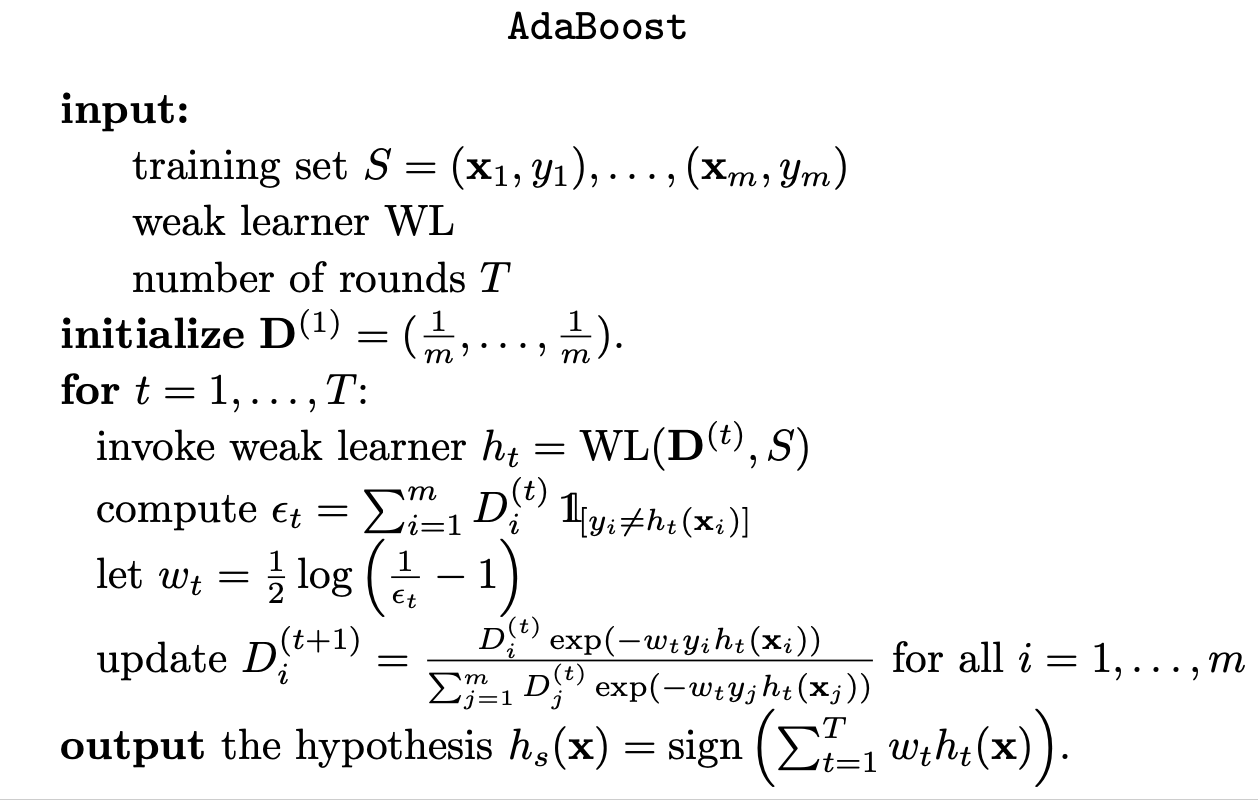
\includegraphics[width=0.6\textwidth]{assets/adaboost.png}
\end{center}
\end{frame}

\begin{frame}{AdaBoost Analysis}
    \begin{block}{Theorem: AdaBoost Training Error Upper Bound}
        $S$ 是一个训练集,假设在 AdaBoost 的每一次迭代中,弱分类器返回的假设满足 $\epsilon_t \leq \frac{1}{2} - \gamma$。则 AdaBoost 输出的最终假设的训练误差满足以下不等式:
        \[
        L_S(h_s) = \frac{1}{m} \sum_{i=1}^{m} \mathbbm{1}[h_s(x_i) \neq y_i] \leq \exp(-2 \gamma^2 T)
        \]
    \end{block}
    证明:
    对于每一轮 $t$,记 $f_t = \sum_{p<t} w_p h_p$,因此 AdaBoost 的输出为 $f_T$。此外,记
\[
Z_t = \sum_{i=1}^{m} \exp(-y_i f_t(x_i))
\]

\end{frame}

\begin{frame}{AdaBoost Analysis}
    注意到对于任何假设都有 $ \mathbbm{1}[h(x) \neq y] \leq \exp(-y h(x))$。因此,训练误差满足:
    \[
    L_S(f_T) \leq Z_T
    \]
    所以我们只需证明 $Z_T \leq \exp(-2 \gamma^2 T)$。为了bound 住 $Z_T$,我们将其重写为:
    \[
    Z_T =  \frac{Z_T}{Z_{T-1}} \cdot \frac{Z_{T-1}}{Z_{T-2}}  \cdots \frac{Z_2}{Z_1} \cdot \frac{Z_1}{Z_0}
    \]
    其中我们使用了 $Z_0 = 1$,因为 $f_0 \equiv 0$。现在我们只需证明对于每一轮 $t$:
    \[
    \frac{Z_{t+1}}{Z_t} \leq \exp(-2 \gamma^2)
    \]
    为了证明上式,首先通过简单的归纳推理可知对于所有的 $t$ 和 $i$都有:
    \[
    D_{i}^{(t+1)} = \frac{\exp(-y_i f_t(x_i))}{\sum_{j=1}^{m} \exp(-y_j f_t(x_j))}
    \]
\end{frame}

\begin{frame}{AdaBoost Analysis}
    因此:
    \[
    \frac{Z_{t+1}}{Z_t} = \frac{\sum_{i=1}^{m} \exp(-y_i f_{t+1}(x_i))}{\sum_{j=1}^{m} \exp(-y_j f_t(x_j))} = \frac{\sum_{i=1}^{m} \exp(-y_i f_t(x_i)) \exp(-y_i w_{t+1} h_{t+1}(x_i))}{\sum_{j=1}^{m} \exp(-y_j f_t(x_j))}
    \]
    \[
    \implies \frac{Z_{t+1}}{Z_t} = \exp(-w_{t+1}) \left(1 - \epsilon_{t+1}\right) + \exp(w_{t+1}) \epsilon_{t+1} = 2 \sqrt{\epsilon_{t+1}(1 - \epsilon_{t+1})}
    \]
    根据我们的假设,$\epsilon_{t+1} \leq \frac{1}{2} - \gamma$。由于函数 $g(a) = a(1 - a)$ 在区间 $[0, \frac{1}{2}]$ 上是单调递增的,我们得到:
    \[
    2 \sqrt{\epsilon_{t+1}(1 - \epsilon_{t+1})} \leqslant 2 \sqrt{\left(\frac{1}{2} - \gamma\right) \left(\frac{1}{2} + \gamma\right)} \leqslant \sqrt{1 - 4 \gamma^2} 
    \]
    因此,$\frac{Z_{t+1}}{Z_t} \leq \exp(-2 \gamma^2)$。\qed
\end{frame}